\chapter{Консенсус в распределенных системах}
В распределенных системах консенсус играет важнейшую роль, позволяя узлам достичь согласованности данных даже в условиях сбоев или недобросовестных участников. Это особенно актуально для многопользовательских игр, где необходимо обеспечить согласованное состояние игрового мира для всех игроков. Рассмотрены ключевые алгоритмы достижения консенсуса и их использование в игровой индустрии.

Paxos (1989 г.) ~\cite{b1}, разработанный Лесли Лэмпортом, является одним из первых и наиболее известных алгоритмов консенсуса. Он обеспечивает согласованность в распределенных системах при наличии частичных отказов и сетевых задержек. Paxos состоит из трех фаз: предложения значения, принятия значения и подтверждения принятого значения. Этот алгоритм гарантирует, что система всегда достигает согласованного состояния, даже если некоторые узлы вышли из строя.

Применение Paxos в играх: используется для репликации игровых данных между серверами, гарантирует, что все игроки видят одинаковое состояние игрового мира, даже в случае отказа одного из серверов, позволяет восстановить данные после сбоя, минимизируя потерю игрового прогресса.

Raft (2014 г.) ~\cite{b2}, разработанный Онгаро и Оустерхутом, был создан как более понятная альтернатива Paxos. Raft структурирует процесс консенсуса вокруг лидера, который принимает решения и реплицирует данные другим узлам. Если лидер выходит из строя, алгоритм выбирает нового лидера.

Особенности Raft: простота реализации по сравнению с Paxos, высокая производительность благодаря централизованному управлению через лидера.

Применение Raft в играх: подходит для серверных систем с репликацией состояния, где один сервер принимает решение, а остальные подтверждают его, обеспечивает быстрое восстановление при сбоях лидера, что минимизирует время простоя.

Practical Byzantine Fault Tolerance (PBFT) (1999 г.)~\cite{b3}, предложенный Кастро и Лисков, является алгоритмом, устойчивым к злоумышленникам и сбоям. Он способен работать при наличии до одной трети вредоносных узлов, что делает его подходящим для распределенных систем, требующих высокой степени доверия.

Суть алгоритма: PBFT обеспечивает согласованность в распределенной системе, даже если часть узлов ведет себя недобросовестно. Алгоритм состоит из трех фаз:
\begin{itemize}
	\item pre-prepare -- лидер (primary) инициирует процесс, отправляя запросы узлам;
	\item prepare -- узлы обмениваются сообщениями для подтверждения корректности данных;
	\item commit -- узлы фиксируют согласие, переходя к следующему состоянию.
\end{itemize}

Для согласия требуется одобрение минимум $2/3$ корректных узлов, что обеспечивает устойчивость при наличии до $1/3$ вредоносных.

Применение в играх: PBFT используется для защиты от читерства и атак в распределенных игровых системах, обеспечивая согласованность игровых данных даже при наличии недобросовестных участников.

\chapter{Архитектуры многопользовательских игр}

\section{Клиент-серверная архитектура}
Клиент-серверная архитектура предполагает, что основная игровая логика выполняется на сервере. Сервер выступает центральным узлом, который управляет игровым процессом, а клиенты подключаются к нему для участия в игре. Клиенты, по сути, представляют собой «упрощенные» визуализационные движки, которые обрабатывают ввод игрока, отображают графику и звук, а также передают информацию на сервер ~\cite{b4}.

Особенностью клиентской части является так называемое предсказание действий игрока, что позволяет минимизировать задержки между действиями игрока и их отображением на экране. Это создает ощущение мгновенной реакции, несмотря на возможные сетевые задержки ~\cite{b4}.

Сервер может быть запущен на выделенной машине (режим выделенного сервера), либо сервер и клиент могут работать на одном устройстве (режим «клиент поверх сервера»). Последний вариант часто используется в однопользовательских режимах игр, где сервер обслуживает единственного клиента ~\cite{b4}.

Игровой цикл в таких играх может быть организован несколькими способами:
\begin{itemize}
	\item клиент и сервер реализуются как отдельные процессы (программы);
	\item клиент и сервер выполняются в виде отдельных потоков в рамках одного процесса;
	\item клиент и сервер работают в одном потоке с единым игровым циклом, что снижает накладные расходы при локальной работе в режиме «клиент поверх сервера».
\end{itemize}

В клиент-серверной архитектуре, где сервер выступает как центральный узел управления, наибольшее применение нашли алгоритмы Paxos и Raft. Они поддерживают согласованное состояние серверов в условиях репликации данных. 

Paxos хорошо подходит для распределенных серверов, так как гарантирует согласованность даже при частичных сбоях системы.

Raft, благодаря своей простоте и структурированности, часто используется для управления состоянием серверных систем с одним лидером, что обеспечивает высокую производительность и минимизацию задержек.

Таким образом, клиент-серверная архитектура выигрывает от использования этих алгоритмов, особенно в играх, где требуется надежная синхронизация данных между серверами для поддержания согласованного игрового процесса.

\section{Peer-to-Peer архитектура}
Peer-to-Peer (P2P) архитектура предполагает, что каждая машина в сети одновременно выполняет функции клиента и сервера. Каждая машина обладает авторитетом (правом управления) над определенными объектами в игровом мире. Для объектов, которыми управляет локальная машина, она действует как сервер. Для всех остальных объектов машина выступает в роли клиента, визуализируя состояние, предоставленное удаленным авторитетом ~\cite{b4}.

Игровой цикл в P2P-архитектуре имеет более простую структуру, напоминая цикл однопользовательской игры. Однако внутренняя реализация усложняется тем, что код должен учитывать два режима работы: локальный объект с полным управлением и «прокси-объект», содержащий минимальное представление состояния удаленного объекта. Для этого часто создаются два типа игровых объектов: полноценные объекты, которыми управляет локальная машина, и их упрощенные прокси-версии ~\cite{b4}.

Дополнительные сложности возникают из-за необходимости передачи авторитета над объектами между машинами. Например, если одна из машин выходит из игры, другие машины должны взять на себя управление ее объектами, когда в игру подключается новая машина, часть объектов может быть передана ей для распределения нагрузки ~\cite{b4}.

Таким образом, архитектура Peer-to-Peer оказывает значительное влияние на структуру игрового цикла и требует дополнительных механизмов для синхронизации и перераспределения данных между участниками сети ~\cite{b4}.

Peer-to-Peer (P2P) архитектура накладывает дополнительные требования к методам консенсуса, так как отсутствует централизованный сервер, а доверие между узлами может быть ограниченным. В таких системах часто используется алгоритм PBFT, который обеспечивает защиту от вредоносных действий отдельных участников. 

PBFT хорошо подходит для P2P-архитектуры, так как: позволяет сохранять согласованность данных даже при наличии до одной трети вредоносных узлов, снижает риск манипуляций состоянием игровых объектов, которыми управляют разные узлы.

Однако из-за высокой вычислительной сложности PBFT применяется преимущественно в системах с небольшим числом участников. Для более масштабных игр возможны гибридные подходы, объединяющие элементы PBFT с централизованными алгоритмами, такими как Raft.

\begin{figure}[H]
	\centering
	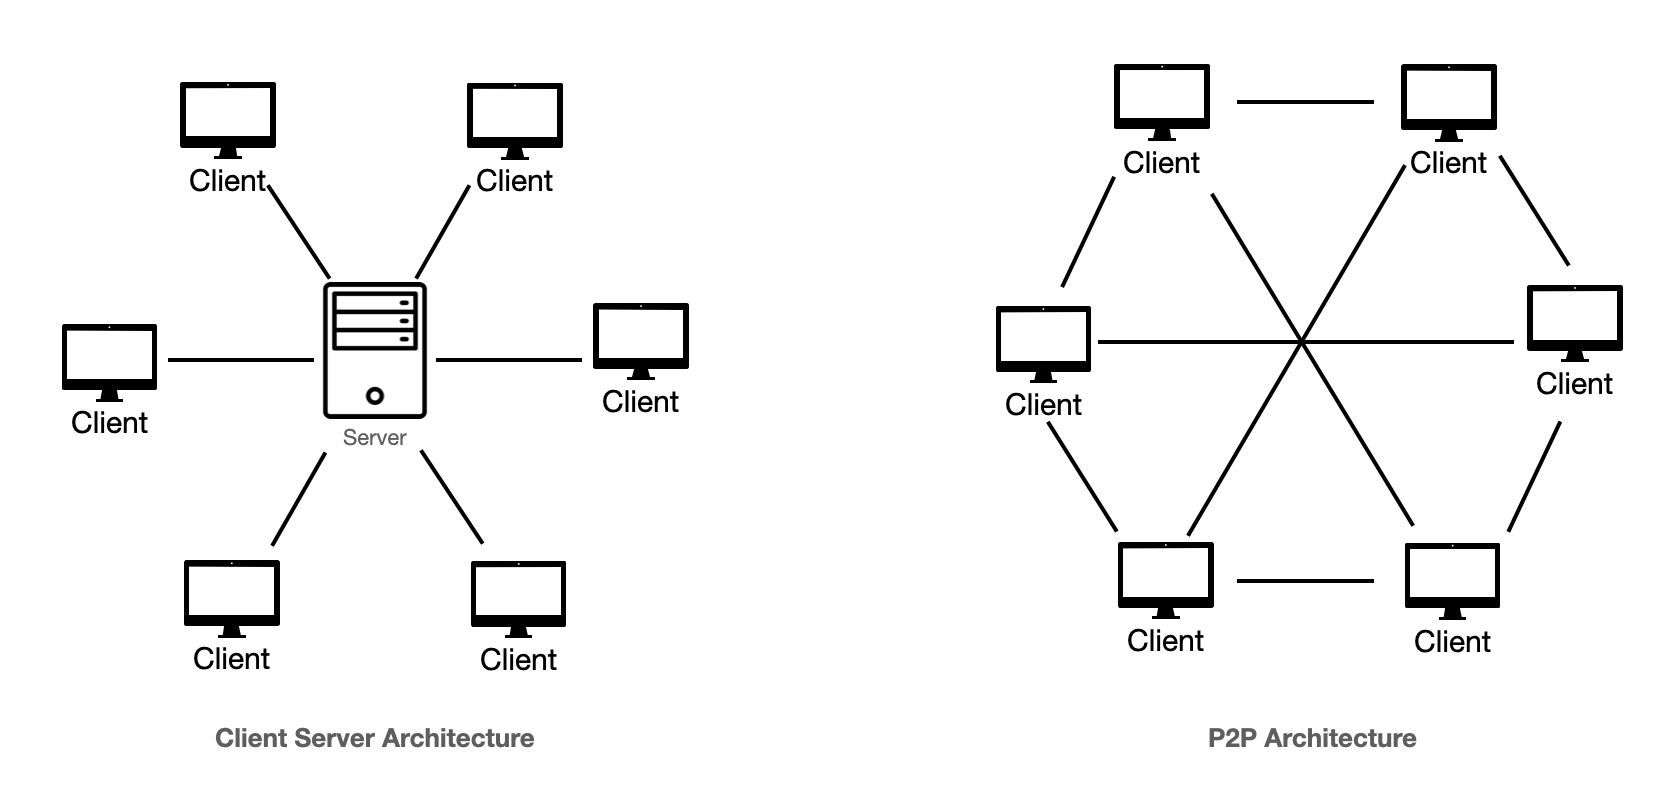
\includegraphics[width=1\textwidth]{img/1.png}
	\caption{Клиент-серверная и P2P архитектуры}
	\label{img:2-1}
\end{figure}

\chapter{Гибридные методы достижения консенсуса}
В современных многопользовательских играх часто используются гибридные методы консенсуса, которые объединяют преимущества различных алгоритмов для повышения эффективности системы. 

В архитектурах, где центральный сервер выполняет критические функции, Raft может использоваться для управления состоянием серверов, а PBFT — для обеспечения согласованности между участниками Peer-to-Peer сети.

Ярким примером применения подобных подходов является игра World of Warcraft (WoW) ~\cite{b8}. В этой MMORPG-игре используется клиент-серверная архитектура с элементами распределенной обработки. Центральные серверы отвечают за хранение и синхронизацию игрового состояния, включая данные об игроках, их взаимодействиях и событиях в мире. Однако локальные данные, такие как действия персонажа, могут временно обрабатываться на стороне клиента для снижения задержек, а затем синхронизироваться с сервером. В критических ситуациях, таких как массовые рейды или PvP-сражения, серверы применяют гибридные стратегии для обеспечения согласованности: часть данных распределяется между региональными узлами, чтобы уменьшить нагрузку, а ключевые события фиксируются на главном сервере.

В играх с распределенной архитектурой центральный сервер может разрешать конфликты, возникающие при достижении консенсуса между узлами, снижая вычислительную нагрузку на каждую отдельную машину.

Такие гибридные подходы особенно актуальны для игр с большим количеством игроков, где требуется одновременно высокая масштабируемость, устойчивость к атакам и надежность обработки данных.

\chapter{Читерство в многопользовательских играх}
Читерство в многопользовательских играх можно определить как любые действия игрока, направленные на получение нечестного преимущества над другими участниками игры, что нарушает правила, установленные разработчиками и игровым сообществом. Читерство приводит к искажению игрового баланса, ухудшению игрового опыта для других игроков и может создавать значительные проблемы для разработчиков.

Примеры атак, связанных с читерством:
\begin{itemize}
	\item подмена данных -- изменение сетевых пакетов для передачи неверной информации серверу или другим клиентам, например, подмена координат, чтобы «телепортировать» персонажа или обходить игровые ограничения;
	\item использование ботов -- создание и использование программ, которые автоматизируют действия игрока, такие как фарм ресурсов, выполнение задач или участие в сражениях;
	\item автоматизация действий -- применение программ или скриптов, ускоряющих реакции игрока (например, автонаведение для стрельбы в шутерах), что невозможно достичь в нормальных условиях.
\end{itemize}

Читерство тесно связано с нарушением консенсуса в многопользовательских играх, особенно в архитектурах, требующих синхронизации данных между клиентами и сервером. В клиент-серверной архитектуре подмена данных на клиентской стороне может привести к рассогласованию с сервером, что нарушает игровой баланс и требует сложных проверок на стороне сервера. В Peer-to-Peer архитектуре злоумышленник может манипулировать состоянием объектов, находящихся под его управлением, что повлияет на игровой процесс для всех участников сети.

Для предотвращения читерства разработчики внедряют различные механизмы защиты, включая верификацию данных на сервере, детектирование ботов с помощью анализа поведения игрока и алгоритмы консенсуса, устойчивые к атакам. Эти меры направлены на восстановление доверия между игроками и обеспечение справедливого игрового процесса.

\section{Анти-читинг технологии}
Анти-читинг технологии -- это совокупность программных и аппаратных решений, предназначенных для предотвращения и выявления читерства в многопользовательских играх. Основная задача таких систем — поддержание честного игрового процесса, защита игроков от злоупотреблений и обеспечение соблюдения игровых правил.

\section{Задачи анти-чит систем}
Основные задачи анти-чит технологий включают:
\begin{itemize}
	\item выявление сторонних программ -- обнаружение приложений, которые могут вмешиваться в игровой процесс или изменять данные;
	\item проверка целостности игровых файлов -- предотвращение модификации клиентской части игры, что может нарушить игровой баланс;
	\item мониторинг поведения игроков -- анализ игрового процесса для выявления подозрительных действий, характерных для ботов или автоматизированных скриптов;
	\item противодействие подмене данных -- защита от изменения сетевых пакетов или передачи недостоверной информации серверу.
\end{itemize}

\section{Примеры технологий}
Наиболее известные анти-читинг технологии включают:
\begin{itemize}
	\item Valve Anti-Cheat (VAC) ~\cite{b5} -- встроенная в платформу Steam ~\cite{b11} система, предназначенная для обнаружения запрещенного ПО. VAC работает на уровне анализа игровых файлов и процессов, автоматически блокируя игроков, если обнаружены нарушения;
	\item Easy Anti-Cheat (EAC) ~\cite{b6} -- популярная система, используемая во многих современных играх. EAC защищает как от известных читов, так и от новых угроз с помощью технологий машинного обучения и поведенческого анализа;
	\item Battleye ~\cite{b7} -- анти-чит технология, применяемая в таких играх, как PUBG ~\cite{b9} и Rainbow Six Siege ~\cite{b10}, фокусируется на предотвращении модификации клиентской части игры и выявлении сетевых атак.
\end{itemize}

\section{Роль анти-чит систем в поддержании консенсуса}
Анти-чит технологии играют ключевую роль в поддержании консенсуса в многопользовательских играх. Они обеспечивают:
\begin{itemize}
	\item целостность данных -- предотвращение изменений клиентских данных, которые могут нарушить согласованное состояние игровых объектов;
	\item честное распределение ресурсов -- блокировка автоматизированных инструментов, которые дают несправедливые преимущества;
	\item доверие между игроками -- устранение угроз, связанных с читерством, способствует созданию честной и конкурентной среды.
\end{itemize}

Эффективность анти-чит систем во многом зависит от своевременного обновления и адаптации к новым видам атак. Системы, такие как VAC, Easy Anti-Cheat и Battleye, демонстрируют, что интеграция комплексных механизмов защиты позволяет существенно снизить уровень читерства и поддерживать справедливость игрового процесса.

\chapter{Критерии оценки методов достижения консенсуса}

Для оценки методов достижения консенсуса в распределенных системах, включая многопользовательские игры, применяются следующие основные критерии:

Продуктивность описывает эффективность метода в условиях высокой нагрузки. В контексте игр это включает: скорость обработки событий в реальном времени, таких как действия игроков или изменение состояния объектов, минимизация задержек при синхронизации данных между участниками сети.

Масштабируемость характеризует способность системы сохранять производительность при увеличении числа участников. В играх это означает: поддержку большого количества игроков без значительного увеличения задержек, эффективную работу в различных сетевых условиях, включая высокую задержку или потерю пакетов.

Устойчивость к атакам описывает способность системы сохранять согласованность данных даже при наличии злоумышленников. Это включает: противодействие попыткам подмены данных, нарушениям консенсуса и другим типам атак, которые могут нарушить нормальный процесс игры.

\chapter{Сравнительный анализ методов консенсуса}

В таблице ниже представлены основные характеристики методов консенсуса, используемых в многопользовательских играх, относительно друг друга:

\begin{center}
	\begin{tabular}{|c|c|c|c|}
		\hline
		Метод & Продуктивность & Масштабируемость & Устойчивость к атакам \\
		\hline
		Paxos & Средняя & Высокая & Средняя \\
		\hline
		Raft & Высокая & Средняя & Средняя \\
		\hline
		PBFT & Средняя & Низкая & Высокая \\
		\hline
	\end{tabular}
\end{center}

Рассмотренные методы консенсуса и архитектуры могут эффективно применяться в многопользовательских играх в зависимости от требований к производительности, устойчивости к атакам и масштабируемости.

